\section{Scintillation Detectors}
\subsection{General Remarks}
\begin{itemize}
    \item Preferred in applications where high efficiency is more important than energy resolution (e.g., medical imaging, Compton suppression).
    \item Available as solids, liquids, and gases; useful in detecting all types of ionizing radiation including fast (organic with H) and slow neutrons (Li, B, Gd). 
\end{itemize}

\subsection{Scintillation Detection Principles and Counters}
\subsubsection{Requirements of Scintillators}
\begin{itemize}
    \item High light/ scintillation/ fluorescence yield
    \item Linear conversion of $\Delta E$ to scintillation photons
    \item Transparent to scintillation photons to minimize self-absorption
    \item Short decay time of fluorescence (ps$\sim$ns) for generation of fast pulses
    \item Good optical quality with sufficient size
    \item Index of refraction $n\sim1.5$ (glass) for efficient coupling to readout device (PMT or other light sensors)
    \item Fluorescence wavelength matches spectral response of readout device
\end{itemize}

\subsubsection{Types of Scintillators}
\begin{enumerate}
    \item Organic
    \begin{itemize}
        \item Liquids, crystals, and plastics
        \item Low Z and low density
        \item Low and \emph{non-linear} light output
        \item Fast decay times
        \item High H content allows fast neutron detection
        \item Pulse-shape discrimination between various particles
    \end{itemize}
    \item Inorganic
    \begin{itemize}
        \item Crystals such as alkali-halide (M$^+$X$^-$)
        \item High Z and high density
        \item High and (relatively) linear light output
        \item Slower decay times
    \end{itemize}
\end{enumerate}
\begin{figure}[ht]
    \centering
    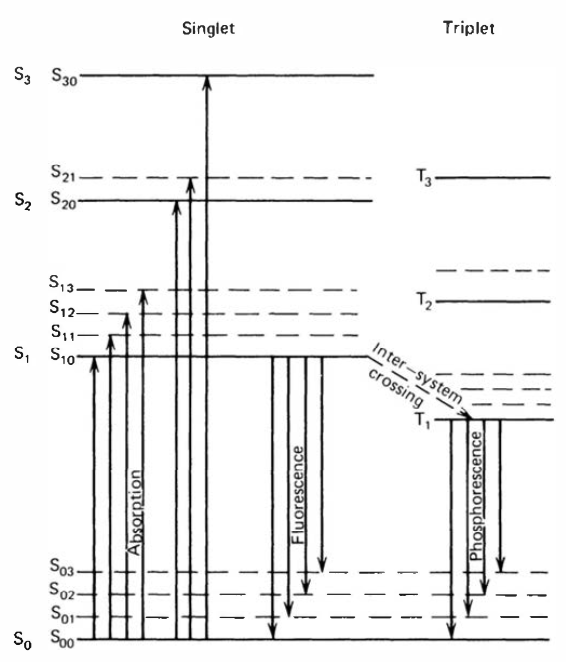
\includegraphics[width=0.4\textwidth]{images/organic_scintillator_energy_level.png}
    \caption{Energy levels of an organic molecule with the $\pi$-electron structure.}
    \label{fig:organic_scintillator_energy_level}
\end{figure}
\subsubsection{Organic Scintillators}
\begin{itemize}
    \item Fluorescence arises from transitions in the energy level structure of a single molecule, independent of physical state (solid, liquid, gas).
    \item The ground state of electrons in the $S_{00}$ singlet state (second index denotes vibration states), and interactions populate higher $S$ states, followed by rapid radiation-less de-excitations into the $S_{10}$ state. Prompt fluorescence is emitted by $S_{10}$ to $S_{0x}$ transitions. See figure~\ref{fig:organic_scintillator_energy_level}.
    \item Some singlet states decay into triplet ($T$) states with much longer lifetimes.
    \item As shown in figure~\ref{fig:organic_scintillator_energy_level}, the $T_1$ to $S_0$ state can be via a delayed light emission characterized as phosphorescence. 
    \item Since the $T_1$ state lies below the $S_0$ state, molecules in the $T_1$ state can be thermally excited back to the $S_1$ state before decaying through normal fluorescence. This is the origin of the delayed fluorescence sometimes observed for organics. 
    \begin{itemize}
        \item The light output is therefore described by a fast component and a slow component:
        \item[] $N=A\exp\left(-\frac{t}{\tau_f}\right)+B\exp\left(-\frac{t}{\tau_s}\right)$
    \end{itemize}
    \item The fact that the fraction of light that appears in the slow component depends on the nature of the exciting particles allows for pulse shape discrimination. Figure~\ref{fig:organic_scintillator_psd} shows the differences in the slow component of various particles with different ionizing density. 
    \begin{figure}[ht]
        \centering
        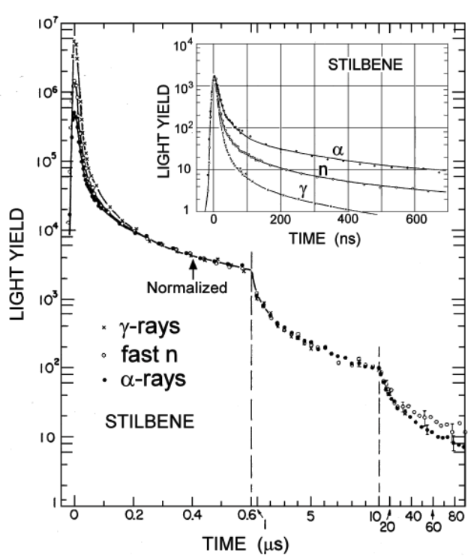
\includegraphics[width=0.4\textwidth]{images/organic_scintillator_psd.png}
        \caption{Pulse-shape discrimination.}
        \label{fig:organic_scintillator_psd}
    \end{figure}
    \item Since energies of the fluorescence transitions (downward arrows in figure~\ref{fig:organic_scintillator_energy_level}) are lower than the photon energies that would be strongly absorbed in the material (upward arrows), there is very little overlap between the optical absorption and emission spectra (Stokes shift). Organic scintillators can therefore be transparent to their own fluorescence emission.
    \item Scintillation efficiency is defined as the fraction of all incident particle energy that is converted into visible light. While we wish to maximize this efficiency, alternate de-excitation modes exist, in which the excitation is degraded mainly into heat. These radiation-less de-excitations are grouped under the term \emph{quenching}.
    \item Linearity between light yield and initial energy builds on the independence of the scintillation efficiency on energy. For organic scintillators, the response to electrons above 125 keV is linear, but for heavy charged particles (proton, alpha), the light yield is not only lower but also non-linear to higher energies, as shown in figure~\ref{fig:organic_scintillator_proton_nonlinear}. 

    \begin{figure}[ht]
        \centering
        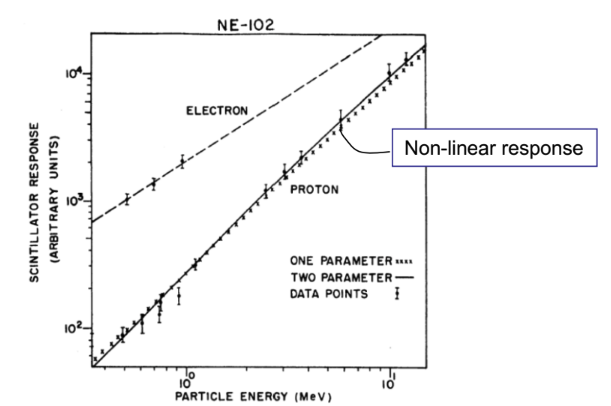
\includegraphics[width=0.5\textwidth]{images/organic_scintillator_proton_nonlinear.png}
        \caption{Non-linearity of light yield in organic scintillators.}
        \label{fig:organic_scintillator_proton_nonlinear}
    \end{figure}
\end{itemize}

\subsubsection{Inorganic Scintillators}


\subsubsection{Comparison of Scintillators}


\subsection{Scintillator Readout}
\subsubsection{Photo-Detectors}
\subsubsection{PMTs}
\subsubsection{Other Multiplication Devices}
\subsection{Scintillator Performance}
\subsubsection{Statistics and Energy Resolution}
\subsubsection{Comparison of Scintillation and HPGe Detectors}
\subsubsection{Limitations of Scintillators}
